\documentclass[twoside]{book}

% Packages required by doxygen
\usepackage{fixltx2e}
\usepackage{calc}
\usepackage{doxygen}
\usepackage[export]{adjustbox} % also loads graphicx
\usepackage{graphicx}
\usepackage[utf8]{inputenc}
\usepackage{makeidx}
\usepackage{multicol}
\usepackage{multirow}
\PassOptionsToPackage{warn}{textcomp}
\usepackage{textcomp}
\usepackage[nointegrals]{wasysym}
\usepackage[table]{xcolor}

% Font selection
\usepackage[T1]{fontenc}
\usepackage[scaled=.90]{helvet}
\usepackage{courier}
\usepackage{amssymb}
\usepackage{sectsty}
\renewcommand{\familydefault}{\sfdefault}
\allsectionsfont{%
  \fontseries{bc}\selectfont%
  \color{darkgray}%
}
\renewcommand{\DoxyLabelFont}{%
  \fontseries{bc}\selectfont%
  \color{darkgray}%
}
\newcommand{\+}{\discretionary{\mbox{\scriptsize$\hookleftarrow$}}{}{}}

% Page & text layout
\usepackage{geometry}
\geometry{%
  a4paper,%
  top=2.5cm,%
  bottom=2.5cm,%
  left=2.5cm,%
  right=2.5cm%
}
\tolerance=750
\hfuzz=15pt
\hbadness=750
\setlength{\emergencystretch}{15pt}
\setlength{\parindent}{0cm}
\setlength{\parskip}{3ex plus 2ex minus 2ex}
\makeatletter
\renewcommand{\paragraph}{%
  \@startsection{paragraph}{4}{0ex}{-1.0ex}{1.0ex}{%
    \normalfont\normalsize\bfseries\SS@parafont%
  }%
}
\renewcommand{\subparagraph}{%
  \@startsection{subparagraph}{5}{0ex}{-1.0ex}{1.0ex}{%
    \normalfont\normalsize\bfseries\SS@subparafont%
  }%
}
\makeatother

% Headers & footers
\usepackage{fancyhdr}
\pagestyle{fancyplain}
\fancyhead[LE]{\fancyplain{}{\bfseries\thepage}}
\fancyhead[CE]{\fancyplain{}{}}
\fancyhead[RE]{\fancyplain{}{\bfseries\leftmark}}
\fancyhead[LO]{\fancyplain{}{\bfseries\rightmark}}
\fancyhead[CO]{\fancyplain{}{}}
\fancyhead[RO]{\fancyplain{}{\bfseries\thepage}}
\fancyfoot[LE]{\fancyplain{}{}}
\fancyfoot[CE]{\fancyplain{}{}}
\fancyfoot[RE]{\fancyplain{}{\bfseries\scriptsize Generated by Doxygen }}
\fancyfoot[LO]{\fancyplain{}{\bfseries\scriptsize Generated by Doxygen }}
\fancyfoot[CO]{\fancyplain{}{}}
\fancyfoot[RO]{\fancyplain{}{}}
\renewcommand{\footrulewidth}{0.4pt}
\renewcommand{\chaptermark}[1]{%
  \markboth{#1}{}%
}
\renewcommand{\sectionmark}[1]{%
  \markright{\thesection\ #1}%
}

% Indices & bibliography
\usepackage{natbib}
\usepackage[titles]{tocloft}
\setcounter{tocdepth}{3}
\setcounter{secnumdepth}{5}
\makeindex

% Hyperlinks (required, but should be loaded last)
\usepackage{ifpdf}
\ifpdf
  \usepackage[pdftex,pagebackref=true]{hyperref}
\else
  \usepackage[ps2pdf,pagebackref=true]{hyperref}
\fi
\hypersetup{%
  colorlinks=true,%
  linkcolor=blue,%
  citecolor=blue,%
  unicode%
}

% Custom commands
\newcommand{\clearemptydoublepage}{%
  \newpage{\pagestyle{empty}\cleardoublepage}%
}

\usepackage{caption}
\captionsetup{labelsep=space,justification=centering,font={bf},singlelinecheck=off,skip=4pt,position=top}

%===== C O N T E N T S =====

\begin{document}

% Titlepage & ToC
\hypersetup{pageanchor=false,
             bookmarksnumbered=true,
             pdfencoding=unicode
            }
\pagenumbering{alph}
\begin{titlepage}
\vspace*{7cm}
\begin{center}%
{\Large My Project }\\
\vspace*{1cm}
{\large Generated by Doxygen 1.8.13}\\
\end{center}
\end{titlepage}
\clearemptydoublepage
\pagenumbering{roman}
\tableofcontents
\clearemptydoublepage
\pagenumbering{arabic}
\hypersetup{pageanchor=true}

%--- Begin generated contents ---
\chapter{S\+T\+V/P Voting System Index Page}
\label{index}\hypertarget{index}{}\hypertarget{index_intro_sec}{}\section{Introduction}\label{index_intro_sec}
This is the introduction. This is an introductory sentence. 
\chapter{Class Index}
\section{Class List}
Here are the classes, structs, unions and interfaces with brief descriptions\+:\begin{DoxyCompactList}
\item\contentsline{section}{\hyperlink{classBallotBox}{Ballot\+Box} }{\pageref{classBallotBox}}{}
\item\contentsline{section}{\hyperlink{classCandidate}{Candidate} }{\pageref{classCandidate}}{}
\item\contentsline{section}{\hyperlink{classCandidates}{Candidates} }{\pageref{classCandidates}}{}
\item\contentsline{section}{\hyperlink{classDriver}{Driver} }{\pageref{classDriver}}{}
\item\contentsline{section}{\hyperlink{classElection}{Election} }{\pageref{classElection}}{}
\item\contentsline{section}{\hyperlink{classReporter}{Reporter} }{\pageref{classReporter}}{}
\end{DoxyCompactList}

\chapter{Class Documentation}
\hypertarget{classBallotBox}{}\section{Ballot\+Box Class Reference}
\label{classBallotBox}\index{Ballot\+Box@{Ballot\+Box}}


Collaboration diagram for Ballot\+Box\+:
\nopagebreak
\begin{figure}[H]
\begin{center}
\leavevmode
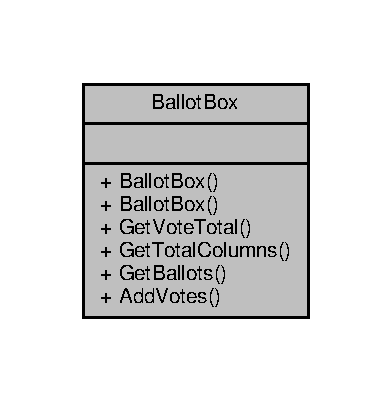
\includegraphics[width=188pt]{classBallotBox__coll__graph}
\end{center}
\end{figure}
\subsection*{Public Member Functions}
\begin{DoxyCompactItemize}
\item 
\mbox{\Hypertarget{classBallotBox_ae1a3df998fab9d6e3d047831f9b68739}\label{classBallotBox_ae1a3df998fab9d6e3d047831f9b68739}} 
{\bfseries Ballot\+Box} (int election\+Type\+\_\+)
\item 
\mbox{\Hypertarget{classBallotBox_a67de3fc3194d03e45f23cb50c5d49f08}\label{classBallotBox_a67de3fc3194d03e45f23cb50c5d49f08}} 
int {\bfseries Get\+Vote\+Total} ()
\item 
\mbox{\Hypertarget{classBallotBox_aa8a05c3bd77b31b6d1845830aff6826e}\label{classBallotBox_aa8a05c3bd77b31b6d1845830aff6826e}} 
int {\bfseries Get\+Total\+Columns} ()
\item 
\mbox{\Hypertarget{classBallotBox_acc0a077b87fb2705e67de17b9263b629}\label{classBallotBox_acc0a077b87fb2705e67de17b9263b629}} 
int $\ast$$\ast$ {\bfseries Get\+Ballots} ()
\item 
\mbox{\Hypertarget{classBallotBox_a54b15e3c3feb53dd4578843a28d418b7}\label{classBallotBox_a54b15e3c3feb53dd4578843a28d418b7}} 
int $\ast$$\ast$ {\bfseries Add\+Votes} (string $\ast$filenames, int file\+Total)
\end{DoxyCompactItemize}


The documentation for this class was generated from the following files\+:\begin{DoxyCompactItemize}
\item 
/home/hans4837/\+C\+S\+C\+I\+\_\+5801/repo-\/\+Team16/src/Ballot\+Box.\+h\item 
/home/hans4837/\+C\+S\+C\+I\+\_\+5801/repo-\/\+Team16/src/Ballot\+Box.\+cpp\end{DoxyCompactItemize}

\hypertarget{classCandidate}{}\section{Candidate Class Reference}
\label{classCandidate}\index{Candidate@{Candidate}}


Collaboration diagram for Candidate\+:
\nopagebreak
\begin{figure}[H]
\begin{center}
\leavevmode
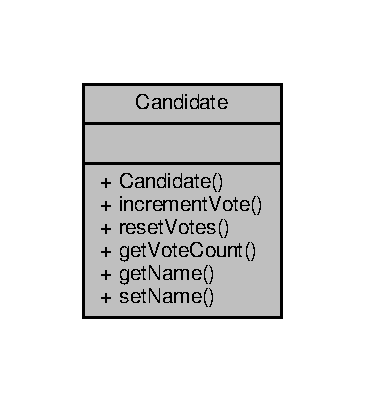
\includegraphics[width=175pt]{classCandidate__coll__graph}
\end{center}
\end{figure}
\subsection*{Public Member Functions}
\begin{DoxyCompactItemize}
\item 
\mbox{\Hypertarget{classCandidate_a99c1eda1eeecf4bbd054049449954c90}\label{classCandidate_a99c1eda1eeecf4bbd054049449954c90}} 
{\bfseries Candidate} (std\+::string name)
\item 
\mbox{\Hypertarget{classCandidate_aebdd30b267da46060d03374cc76c2603}\label{classCandidate_aebdd30b267da46060d03374cc76c2603}} 
void {\bfseries increment\+Vote} ()
\item 
\mbox{\Hypertarget{classCandidate_a2d4e7b4d2e0d32468688e5e4c2c9b098}\label{classCandidate_a2d4e7b4d2e0d32468688e5e4c2c9b098}} 
void {\bfseries reset\+Votes} ()
\item 
\mbox{\Hypertarget{classCandidate_acce26ecaedcc448a3c90b9af5f45dea6}\label{classCandidate_acce26ecaedcc448a3c90b9af5f45dea6}} 
int {\bfseries get\+Vote\+Count} ()
\item 
\mbox{\Hypertarget{classCandidate_af862d92e21d66d74f1d5cae92937d3da}\label{classCandidate_af862d92e21d66d74f1d5cae92937d3da}} 
std\+::string {\bfseries get\+Name} ()
\item 
\mbox{\Hypertarget{classCandidate_afd7bc6e324ab669a9440778680a0a5d3}\label{classCandidate_afd7bc6e324ab669a9440778680a0a5d3}} 
void {\bfseries set\+Name} (std\+::string new\+Name)
\end{DoxyCompactItemize}
\subsection*{Friends}
\begin{DoxyCompactItemize}
\item 
\mbox{\Hypertarget{classCandidate_ab8aa4bfa45d2a47423d3c31bacc7c293}\label{classCandidate_ab8aa4bfa45d2a47423d3c31bacc7c293}} 
bool {\bfseries operator==} (\hyperlink{classCandidate}{Candidate} c1, \hyperlink{classCandidate}{Candidate} c2)
\end{DoxyCompactItemize}


The documentation for this class was generated from the following files\+:\begin{DoxyCompactItemize}
\item 
/home/hans4837/\+C\+S\+C\+I\+\_\+5801/repo-\/\+Team16/src/Candidate.\+h\item 
/home/hans4837/\+C\+S\+C\+I\+\_\+5801/repo-\/\+Team16/src/Candidate.\+cpp\end{DoxyCompactItemize}

\hypertarget{classCandidates}{}\section{Candidates Class Reference}
\label{classCandidates}\index{Candidates@{Candidates}}


Collaboration diagram for Candidates\+:
\nopagebreak
\begin{figure}[H]
\begin{center}
\leavevmode
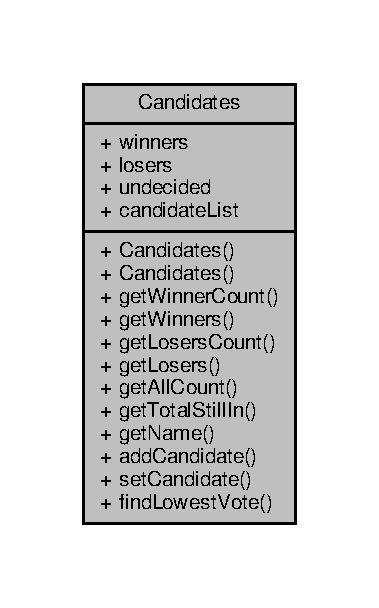
\includegraphics[width=182pt]{classCandidates__coll__graph}
\end{center}
\end{figure}
\subsection*{Public Types}
\begin{DoxyCompactItemize}
\item 
\mbox{\Hypertarget{classCandidates_affbd141eaea1fb26ce3e7162414c6594}\label{classCandidates_affbd141eaea1fb26ce3e7162414c6594}} 
enum {\bfseries Status\+\_\+\+Type} \{ {\bfseries Undecided}, 
{\bfseries Winner}, 
{\bfseries Loser}, 
{\bfseries M\+A\+X\+\_\+\+Status\+\_\+\+Type}
 \}
\end{DoxyCompactItemize}
\subsection*{Public Member Functions}
\begin{DoxyCompactItemize}
\item 
\mbox{\Hypertarget{classCandidates_a01101d31a39bf9ecfac19dfd410a4e2b}\label{classCandidates_a01101d31a39bf9ecfac19dfd410a4e2b}} 
{\bfseries Candidates} (std\+::vector$<$ \hyperlink{classCandidate}{Candidate} $>$ candidates)
\item 
\mbox{\Hypertarget{classCandidates_a5b0d5526b0404d62eacf9508fa0d734a}\label{classCandidates_a5b0d5526b0404d62eacf9508fa0d734a}} 
int {\bfseries get\+Winner\+Count} ()
\item 
\mbox{\Hypertarget{classCandidates_aab9db44b4a11c2f64d9e6906fdc4fd59}\label{classCandidates_aab9db44b4a11c2f64d9e6906fdc4fd59}} 
std\+::vector$<$ \hyperlink{classCandidate}{Candidate} $>$ {\bfseries get\+Winners} ()
\item 
\mbox{\Hypertarget{classCandidates_a60467d71e75d8435ff6df2f2fc4f64ae}\label{classCandidates_a60467d71e75d8435ff6df2f2fc4f64ae}} 
int {\bfseries get\+Losers\+Count} ()
\item 
\mbox{\Hypertarget{classCandidates_a5adad2ad59f565081bc723e03b3ab7c2}\label{classCandidates_a5adad2ad59f565081bc723e03b3ab7c2}} 
std\+::vector$<$ \hyperlink{classCandidate}{Candidate} $>$ {\bfseries get\+Losers} ()
\item 
\mbox{\Hypertarget{classCandidates_a0e1a401227fc4edc7017a555c600ce88}\label{classCandidates_a0e1a401227fc4edc7017a555c600ce88}} 
int {\bfseries get\+All\+Count} ()
\item 
\mbox{\Hypertarget{classCandidates_a1e83512f338373dd37cfdbc1c465ebaf}\label{classCandidates_a1e83512f338373dd37cfdbc1c465ebaf}} 
int {\bfseries get\+Total\+Still\+In} ()
\item 
\mbox{\Hypertarget{classCandidates_a0572a194cae9dd16480de5ecd199994a}\label{classCandidates_a0572a194cae9dd16480de5ecd199994a}} 
std\+::string {\bfseries get\+Name} (int id)
\item 
\mbox{\Hypertarget{classCandidates_aa5a6ed6278777269d02810ff666e8ab5}\label{classCandidates_aa5a6ed6278777269d02810ff666e8ab5}} 
void {\bfseries add\+Candidate} (std\+::string)
\item 
\mbox{\Hypertarget{classCandidates_aa64ba83a526524c5d72666c86e2a0fd5}\label{classCandidates_aa64ba83a526524c5d72666c86e2a0fd5}} 
void {\bfseries set\+Candidate} (std\+::string candidate\+Name, std\+::vector$<$ \hyperlink{classCandidate}{Candidate} $>$ move\+From\+List, std\+::vector$<$ \hyperlink{classCandidate}{Candidate} $>$move\+To\+List)
\item 
\mbox{\Hypertarget{classCandidates_ae8c7d64cda478b622414cd3ba5c172e6}\label{classCandidates_ae8c7d64cda478b622414cd3ba5c172e6}} 
int {\bfseries find\+Lowest\+Vote} ()
\end{DoxyCompactItemize}
\subsection*{Public Attributes}
\begin{DoxyCompactItemize}
\item 
\mbox{\Hypertarget{classCandidates_a524fbccad98042e87cb439ad6a23a121}\label{classCandidates_a524fbccad98042e87cb439ad6a23a121}} 
std\+::vector$<$ \hyperlink{classCandidate}{Candidate} $>$ {\bfseries winners}
\item 
\mbox{\Hypertarget{classCandidates_afa9e0ea758c1ce3480ce370c81d2f2d5}\label{classCandidates_afa9e0ea758c1ce3480ce370c81d2f2d5}} 
std\+::vector$<$ \hyperlink{classCandidate}{Candidate} $>$ {\bfseries losers}
\item 
\mbox{\Hypertarget{classCandidates_a12aafec4ca785542ae4408fbe11c2bd0}\label{classCandidates_a12aafec4ca785542ae4408fbe11c2bd0}} 
std\+::vector$<$ \hyperlink{classCandidate}{Candidate} $>$ {\bfseries undecided}
\item 
\mbox{\Hypertarget{classCandidates_ac7a165f3d34b29981576e63d94ef9e6e}\label{classCandidates_ac7a165f3d34b29981576e63d94ef9e6e}} 
std\+::vector$<$ \hyperlink{classCandidate}{Candidate} $>$ {\bfseries candidate\+List}
\end{DoxyCompactItemize}


The documentation for this class was generated from the following files\+:\begin{DoxyCompactItemize}
\item 
/home/hans4837/\+C\+S\+C\+I\+\_\+5801/repo-\/\+Team16/src/Candidates.\+h\item 
/home/hans4837/\+C\+S\+C\+I\+\_\+5801/repo-\/\+Team16/src/Candidates.\+cpp\end{DoxyCompactItemize}

\hypertarget{classDriver}{}\section{Driver Class Reference}
\label{classDriver}\index{Driver@{Driver}}


Collaboration diagram for Driver\+:\nopagebreak
\begin{figure}[H]
\begin{center}
\leavevmode
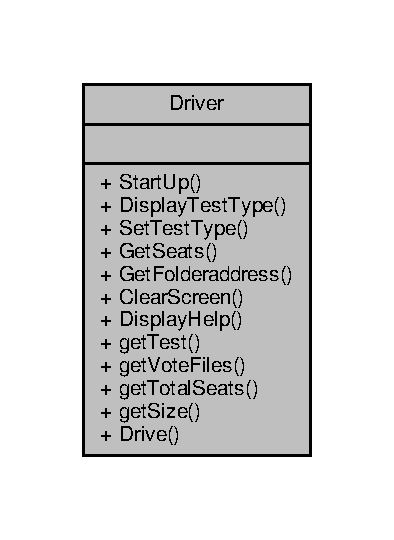
\includegraphics[width=189pt]{classDriver__coll__graph}
\end{center}
\end{figure}
\subsection*{Public Member Functions}
\begin{DoxyCompactItemize}
\item 
\mbox{\Hypertarget{classDriver_a2208d65a809256e174bc0511947d19a5}\label{classDriver_a2208d65a809256e174bc0511947d19a5}} 
void {\bfseries Start\+Up} ()
\item 
void \hyperlink{classDriver_afa66a3ba1778ac080ad30b07f7915daa}{Display\+Test\+Type} ()
\item 
\mbox{\Hypertarget{classDriver_a9110b66fd8fc786047317a5a653c0768}\label{classDriver_a9110b66fd8fc786047317a5a653c0768}} 
void {\bfseries Set\+Test\+Type} (int in)
\item 
\mbox{\Hypertarget{classDriver_acd02a66f92781df2b4c3dad62dad506b}\label{classDriver_acd02a66f92781df2b4c3dad62dad506b}} 
void {\bfseries Get\+Seats} ()
\item 
void \hyperlink{classDriver_a2cd4795b0b07b4018f7c0d4c5d274fa5}{Get\+Folderaddress} ()
\item 
\mbox{\Hypertarget{classDriver_a8207a3147c427f6f5ac04988ad2062ea}\label{classDriver_a8207a3147c427f6f5ac04988ad2062ea}} 
void {\bfseries Clear\+Screen} ()
\item 
\mbox{\Hypertarget{classDriver_ab663de97e197b1f6842a007a31896677}\label{classDriver_ab663de97e197b1f6842a007a31896677}} 
void {\bfseries Display\+Help} ()
\item 
\mbox{\Hypertarget{classDriver_a3f4eae6573765b012d98351df5e5bc5a}\label{classDriver_a3f4eae6573765b012d98351df5e5bc5a}} 
int {\bfseries get\+Test} ()
\item 
\mbox{\Hypertarget{classDriver_a313df2bcb750e2d91bfbe61dfdf32df7}\label{classDriver_a313df2bcb750e2d91bfbe61dfdf32df7}} 
string $\ast$ {\bfseries get\+Vote\+Files} ()
\item 
\mbox{\Hypertarget{classDriver_a0bb8bda66543ae9a662723dfb0a5eca6}\label{classDriver_a0bb8bda66543ae9a662723dfb0a5eca6}} 
int {\bfseries get\+Total\+Seats} ()
\item 
\mbox{\Hypertarget{classDriver_aa3cac88980b5d7c292d1c795086495a8}\label{classDriver_aa3cac88980b5d7c292d1c795086495a8}} 
int {\bfseries get\+Size} ()
\item 
\mbox{\Hypertarget{classDriver_a742a16dbeddf4940c05cc2c6c59dd32f}\label{classDriver_a742a16dbeddf4940c05cc2c6c59dd32f}} 
void {\bfseries Drive} ()
\end{DoxyCompactItemize}


\subsection{Member Function Documentation}
\mbox{\Hypertarget{classDriver_afa66a3ba1778ac080ad30b07f7915daa}\label{classDriver_afa66a3ba1778ac080ad30b07f7915daa}} 
\index{Driver@{Driver}!Display\+Test\+Type@{Display\+Test\+Type}}
\index{Display\+Test\+Type@{Display\+Test\+Type}!Driver@{Driver}}
\subsubsection{\texorpdfstring{Display\+Test\+Type()}{DisplayTestType()}}
{\footnotesize\ttfamily void Driver\+::\+Display\+Test\+Type (\begin{DoxyParamCaption}{ }\end{DoxyParamCaption})\hspace{0.3cm}{\ttfamily [inline]}}

This Method Prompts the user for a specific test type and sets a private variable as that. It takes a case sensitive string from the user and identifies which method is being used. It then moves to setting the testtype. \mbox{\Hypertarget{classDriver_a2cd4795b0b07b4018f7c0d4c5d274fa5}\label{classDriver_a2cd4795b0b07b4018f7c0d4c5d274fa5}} 
\index{Driver@{Driver}!Get\+Folderaddress@{Get\+Folderaddress}}
\index{Get\+Folderaddress@{Get\+Folderaddress}!Driver@{Driver}}
\subsubsection{\texorpdfstring{Get\+Folderaddress()}{GetFolderaddress()}}
{\footnotesize\ttfamily void Driver\+::\+Get\+Folderaddress (\begin{DoxyParamCaption}{ }\end{DoxyParamCaption})\hspace{0.3cm}{\ttfamily [inline]}}

This function is dedicated to getting the folder addresses from the user. It takes in the how many file a user wants, it makes sure that the the user inputs a correct value. The function then makes sure a array has been made and then applys the string names to the user. If a part of this process is incorrect, it returns the user to the main menu or asks the user to reinput data. 

The documentation for this class was generated from the following file\+:\begin{DoxyCompactItemize}
\item 
/home/hans4837/\+C\+S\+C\+I\+\_\+5801/repo-\/\+Team16/\+Project1/src/Driver.\+cpp\end{DoxyCompactItemize}

\hypertarget{classElection}{}\section{Election Class Reference}
\label{classElection}\index{Election@{Election}}


Collaboration diagram for Election\+:\nopagebreak
\begin{figure}[H]
\begin{center}
\leavevmode
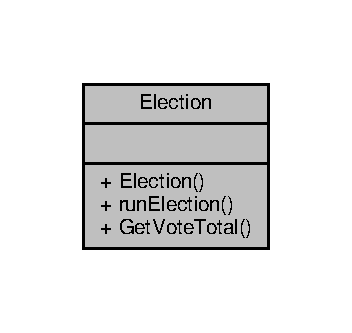
\includegraphics[width=169pt]{classElection__coll__graph}
\end{center}
\end{figure}
\subsection*{Public Member Functions}
\begin{DoxyCompactItemize}
\item 
\mbox{\Hypertarget{classElection_af00d655bcd6df012b8442b1b58f4d6c9}\label{classElection_af00d655bcd6df012b8442b1b58f4d6c9}} 
{\bfseries Election} (bool shufflestatus\+\_\+)
\item 
\mbox{\Hypertarget{classElection_a7d5ab53dbe8b72de6c7442715601c842}\label{classElection_a7d5ab53dbe8b72de6c7442715601c842}} 
void {\bfseries run\+Election} (string $\ast$filenames, int file\+Size, int election\+Type, int seat\+Num)
\item 
\mbox{\Hypertarget{classElection_a1c41b29c48ed8e6c612fe2ba44222b5b}\label{classElection_a1c41b29c48ed8e6c612fe2ba44222b5b}} 
int {\bfseries Get\+Vote\+Total} ()
\end{DoxyCompactItemize}


The documentation for this class was generated from the following files\+:\begin{DoxyCompactItemize}
\item 
/home/hans4837/\+C\+S\+C\+I\+\_\+5801/repo-\/\+Team16/\+Project1/src/Election.\+h\item 
/home/hans4837/\+C\+S\+C\+I\+\_\+5801/repo-\/\+Team16/\+Project1/src/Election.\+cpp\end{DoxyCompactItemize}

\hypertarget{classReporter}{}\section{Reporter Class Reference}
\label{classReporter}\index{Reporter@{Reporter}}


Collaboration diagram for Reporter\+:
\nopagebreak
\begin{figure}[H]
\begin{center}
\leavevmode
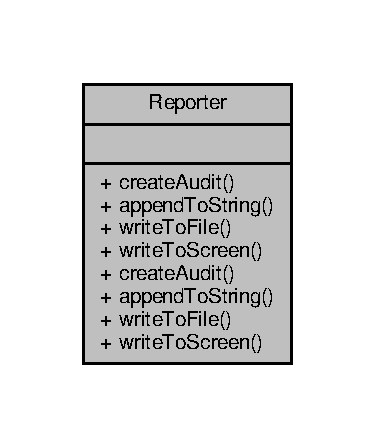
\includegraphics[width=180pt]{classReporter__coll__graph}
\end{center}
\end{figure}
\subsection*{Public Member Functions}
\begin{DoxyCompactItemize}
\item 
\mbox{\Hypertarget{classReporter_a83f740722856a01617c46e05574681ae}\label{classReporter_a83f740722856a01617c46e05574681ae}} 
void {\bfseries create\+Audit} ()
\item 
\mbox{\Hypertarget{classReporter_aa923dc71b57d43ac9c33159d5d250849}\label{classReporter_aa923dc71b57d43ac9c33159d5d250849}} 
void {\bfseries append\+To\+String} (string data)
\item 
\mbox{\Hypertarget{classReporter_a4f98de86ab6d02bace97c8e101109dc1}\label{classReporter_a4f98de86ab6d02bace97c8e101109dc1}} 
void {\bfseries write\+To\+File} (int type, int seats, int candidates, vector$<$ string $>$ winners, vector$<$ string $>$ losers)
\item 
\mbox{\Hypertarget{classReporter_a47c43dfbd9e9319d35a64a4448584dd4}\label{classReporter_a47c43dfbd9e9319d35a64a4448584dd4}} 
void {\bfseries write\+To\+Screen} (int type, int ballots, int seats, int candidates, vector$<$ string $>$ winners, vector$<$ string $>$ losers)
\item 
\mbox{\Hypertarget{classReporter_a83f740722856a01617c46e05574681ae}\label{classReporter_a83f740722856a01617c46e05574681ae}} 
void {\bfseries create\+Audit} ()
\item 
\mbox{\Hypertarget{classReporter_aa923dc71b57d43ac9c33159d5d250849}\label{classReporter_aa923dc71b57d43ac9c33159d5d250849}} 
void {\bfseries append\+To\+String} (string data)
\item 
\mbox{\Hypertarget{classReporter_a4f98de86ab6d02bace97c8e101109dc1}\label{classReporter_a4f98de86ab6d02bace97c8e101109dc1}} 
void {\bfseries write\+To\+File} (int type, int seats, int candidates, vector$<$ string $>$ winners, vector$<$ string $>$ losers)
\item 
\mbox{\Hypertarget{classReporter_a47c43dfbd9e9319d35a64a4448584dd4}\label{classReporter_a47c43dfbd9e9319d35a64a4448584dd4}} 
void {\bfseries write\+To\+Screen} (int type, int ballots, int seats, int candidates, vector$<$ string $>$ winners, vector$<$ string $>$ losers)
\end{DoxyCompactItemize}


The documentation for this class was generated from the following files\+:\begin{DoxyCompactItemize}
\item 
/home/hans4837/\+C\+S\+C\+I\+\_\+5801/repo-\/\+Team16/src/Reporter.\+cpp\item 
/home/hans4837/\+C\+S\+C\+I\+\_\+5801/repo-\/\+Team16/src/Reporter\+Test.\+cpp\end{DoxyCompactItemize}

%--- End generated contents ---

% Index
\backmatter
\newpage
\phantomsection
\clearemptydoublepage
\addcontentsline{toc}{chapter}{Index}
\printindex

\end{document}
